\chapter{Simulação de Sistemas Dinâmicos usando Python} \label{apendice_a}


% Introdução
Nesta apêndice, é apresentado o passo a passo para simulação de sistemas dinâmicos utilizando a linguagem de programação Python e bibliotecas específicas para simulação de sistemas dinâmicos. O pacote \textit{Python Control Systems Library} é utilizado para simular os sistemas dinâmicos, enquanto o \textit{NumPy} é utilizado para a computação científica e o \textit{Matplotlib} para a visualização dos resultados.

\section{Criação de Sistemas}

Neste seção será explorado a criação de sistemas lineares e não lineares. Para isto, é utilizada a função \texttt{control.ss()} da biblioteca \textit{Python Control Systems Library}. A função \texttt{control.ss()} aceita diferentes conjuntos de parâmetros para criar sistemas dinâmicos que serão discutidos a seguir.

\subsection{Sistema Não Lineares}

Para criar um sistema não linear, utiliza-se a opção completa a seguir:

\begin{lstlisting}[language=Python]
  control.ss(updfcn, outfcn, inputs, outputs, states, dt, name, params)
\end{lstlisting}

Essa função cria um sistema de entrada/saída não linear com uma função de atualização \texttt{updfcn} e uma função de saída \texttt{outfcn}. Essa opção é utilizada para especificar um sistema não linear por meio de uma função de atualização de estado e uma função de saída. O sistema pode ser contínuo ou discreto no tempo.

A função \texttt{updfcn(t, x, u, params) $\rightarrow$ \textit{array}} é um objeto \textit{callable} que retorna a função de atualização de estado. Esta função de atualização deve retornar as derivadas dos estados por meio das equações dinâmicas do sistema não linear. Aqui, \texttt{x} é um \textit{array} unidimensional que representa os estados do sistema, \texttt{u} é um \textit{array} unidimensional que representa as entradas do sistema, \texttt{t} é uma variável de ponto flutuante que indica o tempo atual, e \texttt{params} é um dicionário contendo os valores dos parâmetros utilizados pela função. Já a função \texttt{outfcn(t, x, u, params) $\rightarrow$ \textit{array}} é uma função que fornece a saída no estado especificado. Os argumentos são os mesmos que os de \texttt{upfcn}.

\texttt{inputs} descreve as entradas do sistema. Pode ser definido com um valor inteiro que indica a quantidade de entradas do sistema, ou como uma lista de strings que nomeiam os sinais individualmente. Se for definido como um valor inteiro, os nomes dos sinais individuais serão automaticamente definidos como \texttt{u[i]}, onde \texttt{i} é a posição do sinal na lista de entradas do sistema.

\texttt{states} descreve os estados do sistema. Pode ser definido com um valor inteiro que indica a quantidade de estados do sistema, ou como uma lista de strings que nomeiam os sinais individualmente. Se for definido como um valor inteiro, os nomes dos sinais individuais serão automaticamente definidos como \texttt{x[i]}, onde \texttt{i} é a posição do sinal na lista de estados do sistema.

\texttt{outputs} descreve as saídas do sistema. Pode ser definido com um valor inteiro que indica a quantidade de saídas do sistema, ou como uma lista de strings que nomeiam os sinais individualmente. Se for definido como um valor inteiro, os nomes dos sinais individuais serão automaticamente definidos como \texttt{y[i]}, onde \texttt{i} é a posição do sinal na lista de saídas do sistema.

\texttt{name} representa o nome do sistema, o qual pode ser usado para diferenciar os sinais do sistema quando conectado a outros sistemas. Se não especificado, um nome genérico \texttt{<sys[id]>} é gerado com um identificador inteiro único.

\texttt{params} é um dicionário que armazena os valores dos parâmetros necessários para o sistema. Este dicionário é compartilhado com todas as funções de avaliação do sistema.

\subsection{Sistema Lineares}

Os sistemas dinâmicos lineares invariantes no tempo são sistemas que podem ser representados por meio do espaço de estados definidos da seguinte forma: \begin{equation}
  \begin{cases}
    \dt{x}(t) = Ax(t) + Bu(t) \\
    y = Cx(t) + Du(t)
  \end{cases},
  \label{eq:sim_space_model}
\end{equation} onde $x(t) \in \mathbb{R}^{n \times 1}$ é o vetor de estados do sistema, $u(t) \in \mathbb{R}^{m \times 1}$ é o vetor de entradas do sistema, $y(t) \in \mathbb{R}^{l \times 1}$ é o vetor de saídas do sistema, $A \in \mathbb{R}^{n \times n}$ é matriz de estados, $B \in \mathbb{R}^{n \times m}$ é a matriz de entradas, $C \in \mathbb{R}^{l \times n}$ é a matriz de saídas e $D \in \mathbb{R}^{l \times m}$ é a matriz de alimentação.

Dessa forma, para representar um sistema linear invariante no tempo, é possível utilizar a seguinte opção \texttt{control.ss(A, B, C, D[, dt])}. Nesta função, \texttt{A}, \texttt{B}, \texttt{C} e \texttt{D} são \textit{\textit{array}s} que representam as matrizes do sistema \eqref{eq:sim_space_model}, enquanto \texttt{dt} indica se o sistema é contínuo (\texttt{dt = 0}) ou discreto (\texttt{dt > 0}), sendo \texttt{dt} o tempo de amostragem. Esta opção de \texttt{ss()} também aceita os demais parâmetros descritos para a criação de sistemas não lineares na seção anterior, Além disto, é possível criar um sistema linear usando a mesma abordagem da criação de sistemas não lineares por meio das funções \texttt{updfcn} e \texttt{outfcn}, que pode ser útil em determinados casos.

\subsection{Interconexão de sistemas}

Para criar sistemas interconectados utilizando um conjunto de sistemas já criados, é possível utilizar a função \texttt{control.interconnect()}. Esta função aceita os seguinte principais parâmetros: \texttt{syslist}, \texttt{connections}, \texttt{inplist}, \texttt{outlist}, \texttt{inputs}, \texttt{outputs},  \texttt{states} e \texttt{params}.

\texttt{syslist} é a lista de sistemas que serão conectados. O parâmetro \texttt{connections} consiste em uma lista que descreve as conexões internas entre os subsistemas. Cada conexão é representada por uma lista que detalha uma entrada para um dos subsistemas. As conexões podem ser representadas de várias formas, sendo a mais básica por um par ordenado \texttt{('sys', 'sig') or ('sys', 'sig', gain)}, onde \texttt{'sig'} é um sinal de saída que será conectada a entrada \texttt{'sig'} com um ganho \texttt{gain}. Se o ganho for omitido, então ele será considerado igual a 1.

\texttt{inplist} é uma lista de conexões que determina como as entradas para o sistema global são mapeadas para as entradas dos subsistemas. 

\texttt{outlist} é uma lista de conexões que determina como as saídas dos subsistemas são mapeadas para as saídas do sistema global.

\texttt{inputs} descreve as entradas do sistema. Pode ser fornecido como um número inteiro ou como uma lista de strings que nomeiam os sinais individuais. Se fornecido como um número inteiro, os nomes dos sinais serão gerados na forma \texttt{u[i]}.

\texttt{outputs} descreve as saídas do sistema. Pode ser fornecido como um número inteiro ou como uma lista de strings que nomeiam os sinais individuais. Se fornecido como um número inteiro, os nomes dos sinais serão gerados na forma \texttt{y[i]}.

\texttt{states} descreve os estados do sistema. Pode ser fornecido como um número inteiro ou como uma lista de strings que nomeiam os sinais individuais. Se fornecido como um número inteiro, os nomes dos sinais serão gerados na forma \texttt{x[i]}.

4. \texttt{params} é um dicionário que fornece os valores dos parâmetros para os sistemas compartilhado com todas as funções do sistema.

\section{Exemplos}

\subsection{Sistema Massa-Mola}

Considere o seguinte sistema dinâmico massa-mola:

\begin{figure}[H]
  \centering
  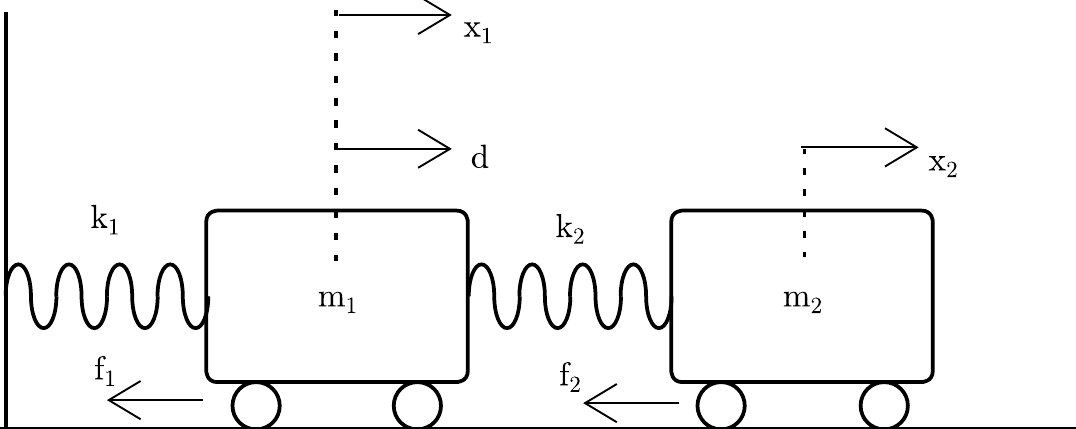
\includegraphics[width=0.8\textwidth]{figuras/sistema_massa_mola.png}
  \caption{Sistema massa-mola.}
  \label{fig:sistema_massa_mola}
\end{figure}

A sua representação no espaço de estados considerando a força $d(t)$ aplicada à massa $m_1$ como sinal de entrada e as posições $x_1(t)$ e $x_2(t)$ como saída do sistema, conforme a seguinte equação: \begin{gather}
  \begin{bmatrix}
    \dot{x_1} \\ \dot{x_2} \\ \ddot{x_1} \\ \ddot{x_2}
  \end{bmatrix}
  =
  \begin{bmatrix}
    0                                   & 0                             & 1                             & 0                             \\
    0                                   & 0                             & 0                             & 1                             \\
    \displaystyle-\frac{k_1 + k_2}{m_1} & \displaystyle\frac{k_2}{m_1}  & \displaystyle-\frac{c_0}{m_1} & 0                             \\
    \displaystyle\frac{k_2}{m_2}        & \displaystyle-\frac{k_2}{m_2} & 0                             & \displaystyle-\frac{c_0}{m_2}
  \end{bmatrix}
  \begin{bmatrix}
    x_1 \\ x_2 \\ \dot{x_1} \\ \dot{x_2}
  \end{bmatrix}
  +
  \begin{bmatrix}
    0                           \\
    0                           \\
    \displaystyle \frac{1}{m_1} \\
    0                           \\
  \end{bmatrix}
  d \\[12pt]
  y =
  \begin{bmatrix}
    1 & 0 & 0 & 0 \\
    0 & 1 & 0 & 0
  \end{bmatrix}
  \begin{bmatrix}
    x_1 \\ x_2 \\ \dot{x_1} \\ \dot{x_2}
  \end{bmatrix}
\end{gather}

Portanto, as matrizes $A$, $B$ e $C$ e $D$ são dadas por: \begin{equation}
  A = \begin{bmatrix}
    0                                   & 0                             & 1                             & 0                             \\
    0                                   & 0                             & 0                             & 1                             \\
    \displaystyle-\frac{k_1 + k_2}{m_1} & \displaystyle\frac{k_2}{m_1}  & \displaystyle-\frac{c_0}{m_1} & 0                             \\
    \displaystyle\frac{k_2}{m_2}        & \displaystyle-\frac{k_2}{m_2} & 0                             & \displaystyle-\frac{c_0}{m_2}
  \end{bmatrix}
  , \space
  B =
  \begin{bmatrix}
    0                           \\
    0                           \\
    \displaystyle \frac{1}{m_1} \\
    0                           \\
  \end{bmatrix}
  , \space
  C =
  \begin{bmatrix}
    1 & 0 & 0 & 0 \\
    0 & 1 & 0 & 0
  \end{bmatrix}
  , \space
  D = 0
\end{equation}

O \autoref{cod:sistema_massa_mola} apresenta um exemplo de como implementar este sistema dinâmico considerando os seguintes valores para parâmetros do sistema: massas $m_1 = 1$ e $m_2 = 0.5$; elasticidade das molas $k_1 = k_2 = 1$; e as forças de atrito $f_1$ e $f_2$ são determinadas por $f_i = -c_0 \cdot \dot{x_i}$, onde $i = 1, 2$. Aqui, $c_0 = 2$ representa o coeficiente de atrito viscoso. E a \autoref{fig:result_sistema_massa_mola} apresenta as figuras obtidas na simulação do sistema massa-mola.

\vspace{8pt}
\begin{lstlisting}[language=Python, caption={Código de simulação do sistema massa-mola.}, label=cod:sistema_massa_mola]
import control as ct
import numpy as np
import matplotlib.pyplot as plt


# Definição dos Parâmetros
m1 = 1.
m2 = 0.5
k1 = 1.
k2 = 1.
c0 = 2.

# Matrizes do sistema massa-mola
A = [
    [0., 0., 1., 0.],
    [0., 0., 0., 1.],
    [-((k1 + k2) / m1), (k2 / m1), - (c0 / m1), 0.],
    [(k2 / m2), - (k2 / m2), 0., - (c0 / m2)]
]

B = [[0.], [0.], [1. / m1], [0.]]

C = [[1, 0, 0, 0], [0, 1, 0, 0]]

D = 0

# Definição do sistema mass-mola
system = ct.ss(
    A, B, C, D,
    name='Sistema Massa-mola',
    inputs=('d'),
    states=('x1', 'x2', 'x1_dot', 'x2_dot'),
    outputs=('x1', 'x2', )
)

# Simulação do sistema

# Tempo de simulação: 0 a 60 segundos, com 100 pontos
timepts = np.linspace(0, 60, 100)

t, y = ct.input_output_response(
    sys=system, T=timepts,
    U=1,
    X0=[0, 0, 0, 0],
)

# Apresentação dos resultados

# Criação e apresentação dos gráficos
fig, axs = plt.subplots(1, 2, figsize=(12, 4))

# Obtenção da saída x1
x1 = y[system.find_output('x1')]

# Gráfico 1 - x1
axs[0].plot(
    t, x1,
    linestyle='-', color='#120a8f', label='$\delta i_L$',
)

axs[0].set_xlabel('Tempo(s)')
axs[0].set_ylabel('Valores de $\delta i_L\,(A)$')
axs[0].set_title('Posição $x_1$')
axs[0].legend()
axs[0].grid(True)

# Obtenção da saída x2
x2 = y[system.find_output('x2')]

# Gráfico 2 - x2
axs[1].plot(
    t, x2,
    linestyle='-', color='#8b0000', label='$\delta v_C$',
)

axs[1].set_xlabel('Tempo(s)')
axs[1].set_ylabel('Valores de $\delta v_C\,(V)$')
axs[1].set_title('Posição $x_2$')
axs[1].legend()
axs[1].grid(True)

fig.suptitle('Sistema Dinâmico Massa-mola', fontsize=16)

plt.tight_layout()
plt.show()

plt.savefig('sistema_massa_mola.eps', format='eps', bbox_inches='tight')

\end{lstlisting}

\begin{figure}[H]
  \centering
  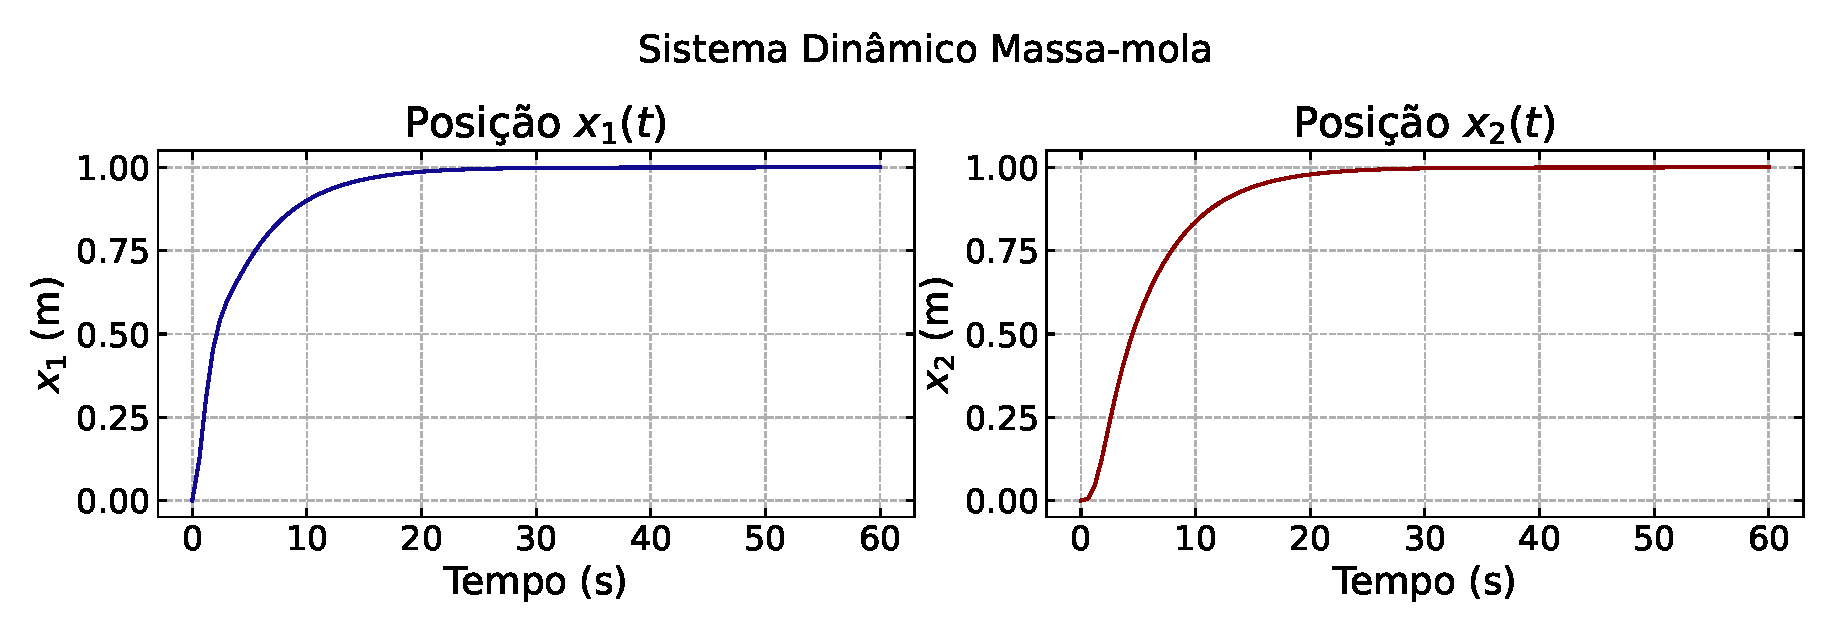
\includegraphics[width=1.\textwidth]{figuras/apendices/A/result.eps}
  \caption{Saídas do sistema massa-mola.}
  \label{fig:result_sistema_massa_mola}
\end{figure}

\subsection{Conversor \acrshort{cc}-\acrshort{cc} \textit{Buck} Não Linear e Linearizado} \label{seção_apendice_a_conversor_buck}

Neste exemplo, é apresentada a implementação e simulação de um Conversor \acrshort{cc}-\acrshort{cc} \textit{Buck} não linear, cujo circuito é ilustrado na figura a seguir:

\begin{figure}[H]
  \centering
  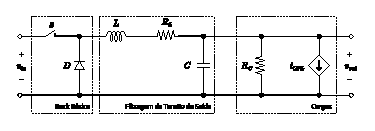
\includegraphics[width=1.\textwidth]{figuras/buck_converter_circuit.eps}
  \captionsetup{justification=centering}
  \caption{Conversor \acrshort{cc}-\acrshort{cc} \textit{Buck} básico com filtragem de tensão de saída conectado a uma \acrshort{crl} e uma \acrshort{cpl}}
  \label{eq:apendice_circuito_buck}
\end{figure}

O seu modelo dinâmico médio não linear é definido como: \begin{equation}\begin{cases} \dt{i}_L &= \displaystyle - \frac{R_L}{L} i_L(t) - \frac{1}{L} v_C(t) + \frac{v_{\mathrm{in}}}{L}d(t)  \\[8pt] \dt{v}_C &= \displaystyle \frac{1}{C} i_L(t) - \frac{1}{C R_C} v_C(t) - \frac{1}{C v_C(t)} P_{\mathrm{cpl}}(t) \label{eq:buck_nonlinear_system} \end{cases}.\end{equation} E seu modelo linearizado em torno do ponto de operação $P_{\mathrm{o}} = \left({i_L}_{\mathrm{o}}, \, {v_C}_{\mathrm{o}}, \, d_{\mathrm{o}}, \, {P_{\mathrm{cpl}}}_{\mathrm{o}} \right)$, onde \begin{equation}\begin{aligned}
    {i_L}_{\mathrm{o}} = \frac{1}{R_C} {v_C}_{\mathrm{o}} + \frac{1}{{v_C}_{\mathrm{o}}} {P_{\mathrm{cpl}}}_{\mathrm{o}} 
     \hspace{1cm}&
    d_{\mathrm{o}} = \frac{R_L}{v_{\mathrm{in}}} {i_L}_{\mathrm{o}} + \frac{{v_C}_{\mathrm{o}}}{v_{\mathrm{in}}}
    \label{eq:operation_point},
  \end{aligned}
\end{equation} é representado pelo seguinte espaço de estados: \begin{equation} \begin{bmatrix} \dt{\delta i_L} \\ \dt{\delta v_C} \end{bmatrix} = \begin{bmatrix} \displaystyle -\frac{R_L}{L} & \displaystyle -\frac{1}{L}  \\[12pt] \displaystyle \frac{1}{C} & \displaystyle \frac{1}{C}\left(\frac{{P_{\mathrm{cpl}}}_{\mathrm{o}}}{{{v_{C}}^2_{\mathrm{o}}}} - \frac{1}{R_C}\right) \end{bmatrix} \begin{bmatrix} \delta i_L(t) \\ \delta v_C(t) \end{bmatrix} + \begin{bmatrix} {\displaystyle \frac{v_{\mathrm{in}}}{L}} & 0 \\[12pt] 0 & \displaystyle {-\frac{1}{C{v_C}_{\mathrm{o}}}} \end{bmatrix}  \begin{bmatrix} \delta d(t) \\ \delta P_{\mathrm{cpl}}(t) \end{bmatrix}. \label{eq:buck_sistema_linearizado}\end{equation} Com base nessas equações, é possível simular o seu comportamento dinâmico computacionalmente, como será apresentados nos próximos passos.

Primeiramente, serão definidos os parâmetros do conversor \textit{Buck} necessários para a sua implementação. Para isto, é criada uma variável \texttt{params} que é um dicionário que conterá os parâmetros do conversor. No conversor \textit{Buck}, os parâmetros são a tensão de entrada (\texttt{Vin}), as resistências (\texttt{rL} e \texttt{rC}), a indutância (\texttt{L}), a capacitância (\texttt{C}), a potência da CPL e a tensão desejada do capacitor (\texttt{Pcpl} e \texttt{vC}). Em seguida, são calculadas a corrente do indutor (\texttt{iL}) e o ciclo de trabalho (\texttt{d}) no ponto de operação, de acordo com as relações expressas em \eqref{eq:operation_point}. Com esses valores do ponto de operação, as entradas \texttt{U\_OP} e os estados \texttt{X\_OP} são definidos. Além disso, a entrada do sistema (\texttt{U}) é definida como os valores no ponto de operação, enquanto os estados iniciais (\texttt{X0}) são definidos como 95\% dos valores no ponto de operação. Por fim, são calculadas as variações nas entradas (\(\delta U\)) e nos estados iniciais ($\delta X0$) em relação ao ponto de operação. A definição completa dos parâmetros do conversor \textit{Buck} está implementada no código a seguir:

\vspace{8pt}
\begin{lstlisting}[language=Python, caption={Parâmetros do conversor \textit{Buck}.}, label=cod:buck_params]
  # Parâmetros do Circuito
  params = {'Vin': 48, 'rL': 0.1, 'rC': 35,
            'L': 40e-3, 'C': 10e-6, 'op': {'Pcpl': 15, 'vC': 24}}

  # Cálculo da Corrente e Duty Cycle de Operação
  op = params['op']
  IL_OP = (op['vC'] / params['rC']) + op['Pcpl'] / op['vC']
  D_OP = (params['rL'] * IL_OP) / params['Vin'] + op['vC'] / params['Vin']

  params['op']['iL'] = IL_OP
  params['op']['d'] = D_OP

  # Ponto de operação de cada entrada e estado do sistema
  U_OP = np.\textit{array}([params['op']['d'], params['op']['Pcpl']])
  X_OP = np.\textit{array}([params['op']['iL'], params['op']['vC']])

  # Entradas do Sistema
  D = params['op']['d']
  P_CPL = params['op']['Pcpl']
  U = np.\textit{array}([D, P_CPL])

  # Estados Iniciais do Sistema
  IL_INIT = 0.95 * params['op']['iL']
  VC_INIT = 0.95 * params['op']['vC']
  X0 = np.\textit{array}([IL_INIT, VC_INIT])

  δU = U - U_OP
  δX0 = X0 - X_OP
\end{lstlisting}

% Implementação do \textit{Buck} não linear
No código \ref{cod:buck_nonlinear}, é apresentada a implementação da função de atualização dos estados e da função de saída do conversor \textit{Buck}, além da criação de um objeto que representa o sistema dinâmico. A função \texttt{update\_buck\_nonlinear} estabelece o comportamento dinâmico do conversor \textit{buck} não linear conforme expresso em \eqref{eq:apendice_circuito_buck}. Esta função recebe como entrada o tempo \texttt{t}, os estados do sistema \texttt{x}, as entradas do sistema \texttt{u} e os parâmetros do sistema \texttt{params}. A partir dessas informações, são calculadas as derivadas dos estados do sistema, que representam as mudanças da corrente do indutor \texttt{diL} e da tensão do capacitor \texttt{dvC}. Além disso, a função \texttt{output\_buck\_nonlinear} é responsável por definir quais variáveis do sistema serão consideradas como saídas, recebendo os mesmos parâmetros da função de atualização dos estados. Dessa forma, ela retorna um vetor com as variáveis de interesse, neste caso, a corrente do indutor \texttt{iL} e a tensão do capacitor \texttt{vC}. Por fim, a variável \texttt{nonlinear\_system} define um sistema de tempo contínuo utilizando a função \texttt{ct.ss}.

\vspace{8pt}
\begin{lstlisting}[language=Python, caption={Implementação do conversor \textit{Buck} não linear.}, label=cod:buck_nonlinear]
def update_buck_nonlinear(t, x, u, params):
  # Parâmetros do sistema
  V_IN = params.get('Vin')  # Tensão de Entrada
  RL = params.get('rL')     # Resistência (indutor)
  RC = params.get('rC')     # Resistência (capacitor)
  L = params.get('L')       # Indutância
  C = params.get('C')       # Capacitância

  # Entradas do sistema: Duty Cycle e Potência da CPL
  D, P_CPL = u

  # Estados do sistema: corrente do indutor e tensão do capacitor
  IL, VC = x

  # Atualização da corrente do indutor
  diL = (V_IN / L) * D - (RL / L) * IL - VC / L  

  # Atualização da tensão do capacitor   
  dvC = IL / C - VC / (C * RC) - P_CPL / (C * VC)

  dx = np.\textit{array}([diL, dvC])
  return dx

# Definição da saída do sistema
def output_buck_nonlinear(t, x, u, params):
  return x[0:2]

# Definição do conversor cc-cc \textit{buck} nao-linear
buck_nonlinear = ct.ss(
  update_buck_nonlinear, 
  output_buck_nonlinear,
  name='buck_nonlinear',
  inputs=('d', 'P_cpl'),
  outputs=('iL', 'vC'),
  states=('iL', 'vC')
)
\end{lstlisting}

O código \ref{cod:buck_linear} implementa a linearização do conversor \textit{Buck} em torno do ponto de operação $P_o$. A variável \texttt{OP} armazena os valores de $P_o$ contida no dicionário \texttt{params} e, portanto, representa o ponto de operação do conversor. Em seguida, são construídas as matrizes de estado \texttt{A}, de entrada \texttt{B}, de saída \texttt{C} e de alimentação \texttt{D} do sistema, de acordo com a linearização do conversor \textit{Buck} definida. Por último, a variável \texttt{buck\_linearized} é criada por meio da transformação do sistema linear, construído com base nas matrizes do sistema, para sua forma de representação entrada-saída. Isso é feito para aumentar a flexibilidade da simulação, permitindo a definição de tags para as entradas, saídas e estados, o que facilita a interconexão entre os sistemas.

\vspace{8pt}
\begin{lstlisting}[language=Python, caption={Implementação do conversor \textit{Buck} linearizado.}, label=cod:buck_linear]
  # Obtenção dos valores no ponto de operação (OP)
  OP = params['op']

  # Elementos da matriz de estados
  A11 = - (params['rL'] / params['L'])
  A12 = - (1. / params['L'])
  A21 = 1. / params['C']
  A22 = (1. / params['C']) * (OP['Pcpl'] /
        (OP['vC'] * OP['vC']) - 1. / params['rC'])

  # Elementos da matriz de entrada
  B11 = params['Vin'] / params['L']
  B12 = 0.
  B21 = 0.
  B22 = - 1.0 / (params['C'] * OP['vC'])

  # Matriz de estados: iL e vC
  A = [[A11, A12], [A21, A22]]

  # Matriz de entradas: d e P_cpl
  B = [[B11, B12], [B21, B22]]

  # Matriz de saída: iL e vC
  C = [[1., 0], [0., 1]]

  # Matriz de alimentação: nula
  D = [[0., 0.], [0., 0.]]

  \textit{Buck}_linearized = ct.ss(
    A, B, C, D,
    name='buck_linearized',
    inputs=('δd', 'δPcpl'),
    outputs=('δiL', 'δvC'),
    states=('δiL', 'δvC')
  )
\end{lstlisting}

\subsection{Conversor \textit{Buck} \acrshort{cc}-\acrshort{cc} em Malha Fechada sob \acrshort{etc}}

Neste exemplo será detalhado a implementação do conversor \textit{Buck} linearizado, definido no exemplo anterior, em malha fechada sob o \acrshort{etc}. Para isto, é realizada a interconexão entre a planta (conversor \textit{Buck}), o \acrshort{etm}, o \acrshort{zoh} e o controlador por realimentação de estados.

A partir dos parâmetros de projetos obtidos por meio da abordagem proposta neste trabalho, é implementado o \acrshort{etm} estático, cujo código está apresentado em \ref{cod:static_etm}. Este possui quatro entradas, das quais as duas primeiras são os últimos estados enviados $\hat{x}$ provenientes do ZOH e os estados atuais $x$ obtidos da planta. Suas saídas consistem em $\Gamma$, uma variável \textit{booleana} que, quando verdadeira, aciona um evento, e os estados atuais da planta. Essas saídas são determinadas pela função \texttt{etm\_output}, a qual recebe como parâmetros o tempo atual da simulação, o estado atual do \acrshort{etm}, a entrada do \acrshort{etm} e os parâmetros do sistema, respectivamente.

Internamente, a função verifica o início da segunda simulação. Isso se deve ao fato de que a simulação é realizada duas vezes: a segunda vez com um passo de simulação maior e menos preciso. Esta distinção é crucial, pois o tempo de acionamento de eventos é registrado apenas na primeira simulação, que utiliza um passo de tempo menor e mais preciso. Além disso, o cálculo de $\Gamma$ é realizado, sendo este um valor real. Caso seja negativo, um novo evento deve ser acionado. Se isso ocorrer, os estados atuais serão definidos como a saída do \acrshort{etm}; caso contrário, serão os últimos estados enviados.

\vspace{8pt}
\begin{lstlisting}[language=Python, caption={Implementação do \acrshort{etm} estático.}, label=cod:static_etm]
  zero = 0
  event_times = [0.]

  def get_gama(current_states, last_states_sent):
    error = last_states_sent - current_states
    return current_states.T @ Ψ @ current_states - error.T @ Ξ @ error


  def etm_output(t, x, u, params):
    global zero, event_times

    if t != etm_output.previous_time:
      etm_output.previous_time = t
      if etm_output.first_simulation and t == 0.:
        etm_output.first_simulation = False

    last_states_sent = u[0:2]
    current_states = u[2:4]

    Γ = get_gama(current_states, last_states_sent)
    trigger = Γ < 0

    if etm_output.first_simulation and trigger:
      event_times.append(t)

    state_to_sent = (current_states if trigger or t == 0. else last_states_sent)
    return [state_to_sent[0], state_to_sent[1]]

  etm_output.previous_time = 0
  etm_output.first_simulation = True

  ETM = ct.ss(
    None, etm_output,
    name='etm',
    inputs=('x1_hat', 'x2_hat', 'x1', 'x2'),
    outputs=('x1', 'x2'),
  )
\end{lstlisting}

No caso do \acrshort{etm} dinâmico, uma nova função, \texttt{etm\_update}, é criada. Esta função é responsável pela atualização da variável dinâmica $\eta$ do \acrshort{etm} dinâmico. Na função de saída, a lei de acionamento é modificada para incorporar a versão dinâmica do \acrshort{etm}. Além disso, uma nova saída do \acrshort{etm} é adicionada, representando a variável dinâmica do próprio \acrshort{etm}. Por fim, tanto a função de atualização quanto a saída do \acrshort{etm} dinâmico dependem dos parâmetros $\theta$ e $\epsilon$, que são previamente definidos.

\vspace{8pt}
\begin{lstlisting}[language=Python, caption={Implementação do \acrshort{etm} dinâmico.}, label=cod:dynamic_etm]
  θ = 1.
  λ = .1
  
  def etm_update(t, n, u, params):
    Γ = get_gama(current_states=u[2:4], last_states_sent=u[0:2])
    dn = -λ * n + Γ
    return [dn]


  def etm_output(t, n, u, params):
    global zero, event_times

    if t != etm_output.previous_time:
      etm_output.previous_time = t
      if etm_output.first_simulation and t == 0.:
        etm_output.first_simulation = False

    last_states_sent = u[0:2]
    current_states = u[2:4]

    Γ = get_gama(current_states, last_states_sent)
    trigger = (n + θ * Γ) < 0

    if etm_output.first_simulation and trigger:
      event_times.append(t)

    state_to_sent = (current_states if trigger or t == 0. else last_states_sent)
    return [state_to_sent[0], state_to_sent[1], n[0]]


  etm_output.previous_time = 0
  etm_output.first_simulation = True

  ETM = ct.ss(
    etm_update, etm_output,
    name='etm',
    states=('n'),
    inputs=('x1_hat', 'x2_hat', 'x1', 'x2'),
    outputs=('x1', 'x2', 'n'),
  )
  \end{lstlisting}

O código \ref{cod:zoh} é a implementação do \acrshort{zoh}. Inicialmente, é definida uma função chamada \texttt{zoh\_output}, que implementa a saída do \acrshort{zoh} para o sistema de controle contínuo. O método de saída \acrshort{zoh} retém o valor de entrada atual até o próximo instante. A função armazena o estado anterior \texttt{previous} e o tempo anterior \texttt{previous\_time}. Em cada chamada, se o tempo atual \texttt{t} for diferente do tempo anteriormente armazenado, o estado anterior é atualizado e o tempo anterior é atualizado para \texttt{t}. A função retorna os estados previamente armazenados \texttt{last\_states\_sent} que é inicializada com os valores iniciais dos estados da planta.

\vspace{8pt}
\begin{lstlisting}[language=Python, caption={Implementação do \acrshort{zoh}}, label=cod:zoh]
  def zoh_output(t, x, u, params):
    if t != zoh_output.previous_time:
      zoh_output.last_states_sent = zoh_output.previous
      zoh_output.previous_time = t
    zoh_output.previous = u
    return zoh_output.last_states_sent

  zoh_output.previous_time = 0
  zoh_output.second_simulation = False
  zoh_output.previous = []
  zoh_output.last_states_sent = δX0.tolist()

  ZOH = ct.ss(
    None, zoh_output,
    name='zoh',
    inputs=('x1', 'x2'),
    outputs=('x1_hat', 'x2_hat'),
  )
\end{lstlisting}

No código \ref{cod:controller}, é definida a função de saída do controlador, \texttt{control\_output}, responsável por implementar a operação de controle para a planta. Dentro dessa função, ocorre o cálculo do ciclo de trabalho, que consiste no produto escalar entre a matriz de ganho $K$ e os estados $\hat{x}$. Assim, a matriz de ganho representada pela variável \texttt{K} é aplicada aos estados representados por \texttt{u}, resultando no cálculo do ciclo de trabalho desejado. Este último é então retornado como saída do controlador. A seguir, é definido o sistema de controle \texttt{CONTROL}. Este sistema é estático (determinado por \texttt{None}) e utiliza a função \texttt{control\_output} como função de saída. O sistema conta com duas entradas, que correspondem aos estados provenientes do \acrshort{zoh}, e uma saída, que representa o ciclo de trabalho, entrada da planta.

\vspace{8pt}
\begin{lstlisting}[language=Python, caption={Implementação do controlador.}, label=cod:controller]
  def control_output(t, x, u, params):
    duty_cycle = K @ u
    return [duty_cycle]


  CONTROL = ct.ss(
      None, control_output,
      name='control',
      inputs=('x1_hat', 'x2_hat'),
      outputs=('u'),
  )
\end{lstlisting}

O código \ref{cod:closed_loop} cria um sistema de controle em malha fechada para o conversor \textit{Buck} sob o \acrshort{etc}. É utilizada a função \texttt{interconnect} para conectar os quatro subsistemas: o sistema linearizado do conversor \textit{Buck}, o \acrshort{etm}, o \acrshort{zoh}, e o controlador. As conexões entre esses componentes são especificadas para formar um loop de realimentação, conforme apresentado na subseção \ref{subsection:etc}. O sistema resultante é então nomeado como \texttt{closed\_loop\_buck\_system}, e suas entradas e saídas são definidas. Em seguida, define-se o tempo de simulação e o sinal de entrada, que neste caso é um sinal constante chamado \texttt{\ensuremath{\delta}Pcpl}, mas também pode ser um vetor contendo valores variados. Por fim, a função \texttt{input\_output\_response} é utilizada para simular a resposta do sistema fechado ao longo do tempo, armazenando as respostas do sistema em \texttt{t} (tempo) e \texttt{y} (saídas do sistema).

\vspace{8pt}
\begin{lstlisting}[language=Python, caption={Sistema em loop fechado sob o ETC.}, label=cod:closed_loop]
  CLOSED_LOOP_BUCK_SYSTEM = ct.interconnect(
      (buck_linearized, ETM, ZOH, CONTROL),
      connections=(
          # Conexão entre a saída do controlador e a planta
          ('buck_linearized.δd', 'control.u'),

          # Conexão entre as saídas do ZOH e da planta ao ETM
          ('etm.x1_hat', 'zoh.x1_hat'),
          ('etm.x2_hat', 'zoh.x2_hat'),
          ('etm.x1', 'buck_linearized.δiL'),
          ('etm.x2', 'buck_linearized.δvC'),

          # Conexão da saída do ETM no ZOH
          ('zoh.x1', 'etm.x1'),
          ('zoh.x2', 'etm.x2'),

          # Conexão da saída do ZOH no controlador
          ('control.x1_hat', 'zoh.x1_hat'),
          ('control.x2_hat', 'zoh.x2_hat'),
      ),
      name='closed_loop_buck_system',
      inplist=('buck_linearized.δPcpl'),
      outlist=('buck_linearized.δiL',
              'buck_linearized.δvC',
              'etm.Γ',
              'buck_linearized.δd',
              ),
      output=('δiL', 'δvC', 'Γ', 'u')
  )

  print(CLOSED_LOOP_BUCK_SYSTEM)
  print('')

  step = 1e-6
  timepts = np.arange(0, 1. + step, step)

  # Simulação para a pertubação constante
  δPcpl = 0.

  t, y = ct.input_output_response(
      sys=CLOSED_LOOP_BUCK_SYSTEM, T=timepts,
      U=δPcpl,
      X0=δX0,
      solve_ivp_method='RK45',
      solve_ivp_kwargs={'max_step': step}
  )
\end{lstlisting}